\section{Numerical Computation by Simulation}
\label{sec:numerical}

It may be possible that one wishes to compute distributions, on
irregular regions, for which there is no closed form solution.
Numerically it is straight-forward to calculate the function
$g(t)$. There are two obvious approaches:
\begin{itemize}

\item Numerical computation of a $n$-dimensional integral over
  $\Omega$, or

\item Simulation of the problem, and estimation of the density from
  simulated results. 

\end{itemize}
The two approaches have different advantages and disadvantages. The
former approach has no stochastic component, and so errors are
predictable and regular. 

The later approach allows complex, potentially non-convex,
non-uniform, problems to be solved as long as they can be
simulated. Given the stochastic nature of the latter, it may help to
say a little more:

The general process is as follows:
\begin{enumerate}

\item Simulate a set of $2N$ points in the region of interest, and
  calculate the distances between successive pairs. The region may be
  irregular, or even non-convex; decisions may be made about some
  lines being inadmissable (because, for instance, they are exterior
  to the region for a non-convex region), or distances may be
  non-Euclidean, or the point distribution can be non-uniform. All
  that is needed is a set of output distances $\{ t_i \}_{i=1}^{N}$.

\item The density could then be approximate through binning, or a
  kernal smoothing technique, but in fact, we don't need direct access
  to the density as the estimator uses the Laplace transform.

\end{enumerate}

We have tested the above approach, running it 30 times (with different
seeds), in Matlab for various values of $N$. The results are shown in
Figure~\ref{fig:simulated_laplace}. The first plot shows estimates of
the mean relative absolute error of the estimated Laplace transforms
over the range $S \in [0, 50]$. We can see from the fitted straight
line, that the errors decrease as $1/\sqrt{N}$, dropping to around 1\%
at around $N=100,000$.


....





The second plot shows the computation times\footnote{Both algorithms
  were implemented in Matlab, the exact method using Matlab's {\tt
    quadqk} function. } relative to the computation times for the
``exact'' method\footnote{Note that both techniques are in some
  respect numerical, because even when we have a closed form solution
  for the density, we still typically need to numerically integrate
  this to obtain the Laplace transform, but we shall refer to this
  solution as ``exact'' for the sake of clarity in the following
  results, and because in the following we perform numerical
  integration with error tolerances of $10^{-6}$, which means the
  errors in this approach are significantly smaller than those of the
  simulation-based approach, at least for the ranges of $N$ tested
  here.}  We can immediately notice that computation times are roughly
linear in $N$, as one might expect. that around the range $N=100,000$,
the simulation approach is competitive with the exact approach.

The simulation-based approach is not as accurate as the exact
numerical approach, however, it accuracy should be sufficient for most
estimation problems, without increasing the computational workload
unduly.
make



\begin{figure}[tbp]
  \begin{center}
    \subfloat[line]{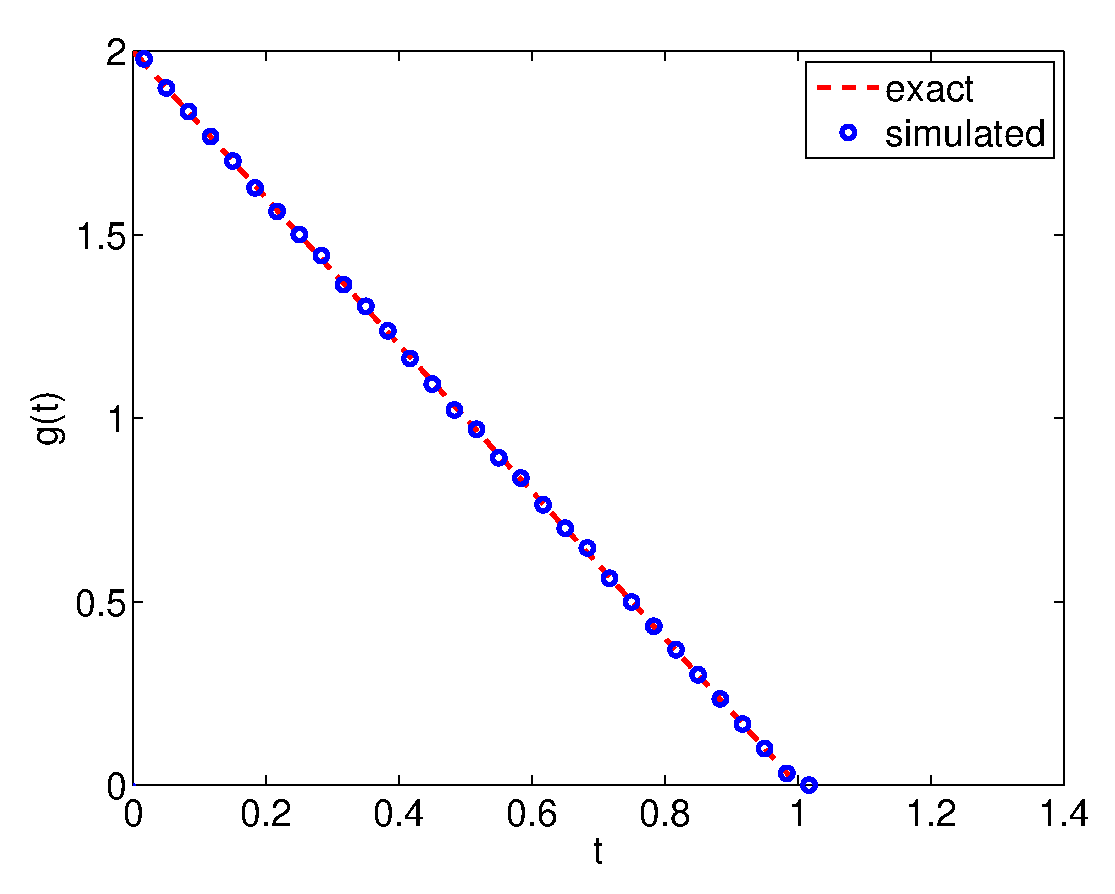
\includegraphics[width=0.32\columnwidth]{../Matlab/Plots/LinePicking_test_sim_line.eps}} 
    \subfloat[square]{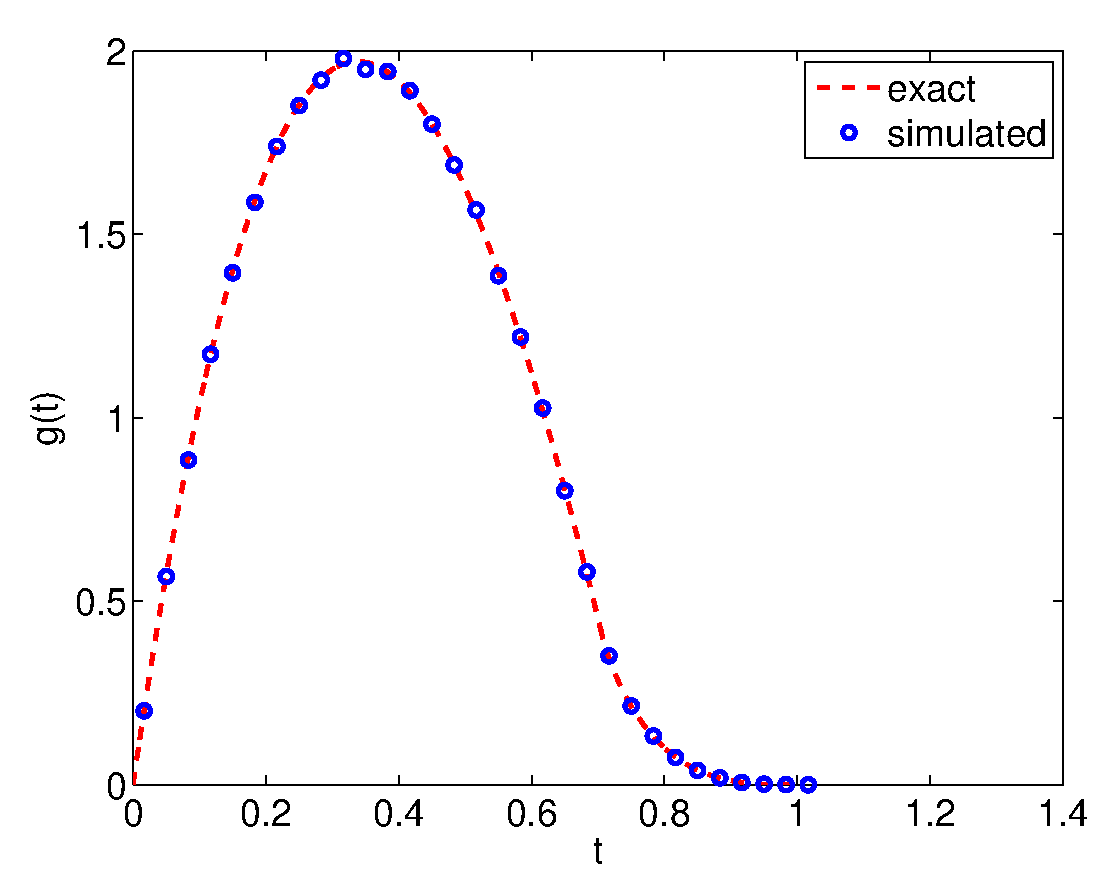
\includegraphics[width=0.32\columnwidth]{../Matlab/Plots/LinePicking_test_sim_square.eps}} 
    \subfloat[rect]{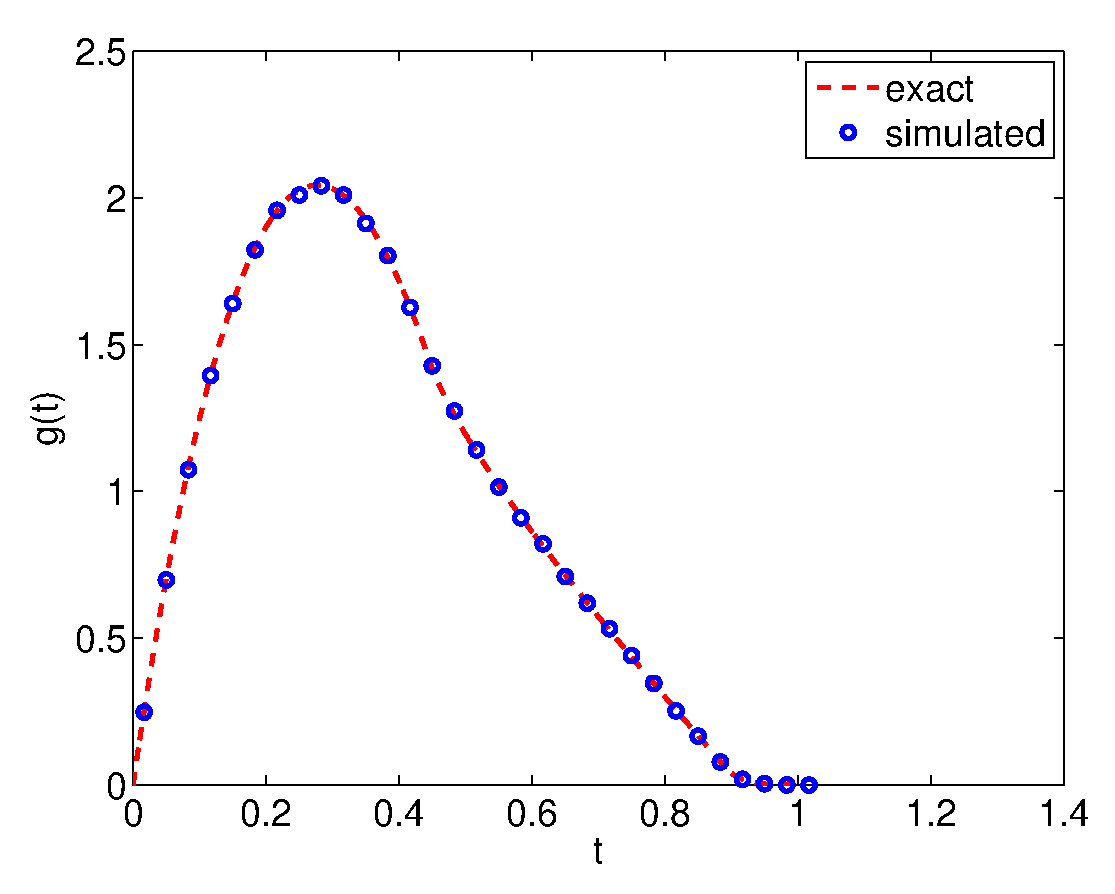
\includegraphics[width=0.32\columnwidth]{../Matlab/Plots/LinePicking_test_sim_rect.eps}} 

    \subfloat[cube]{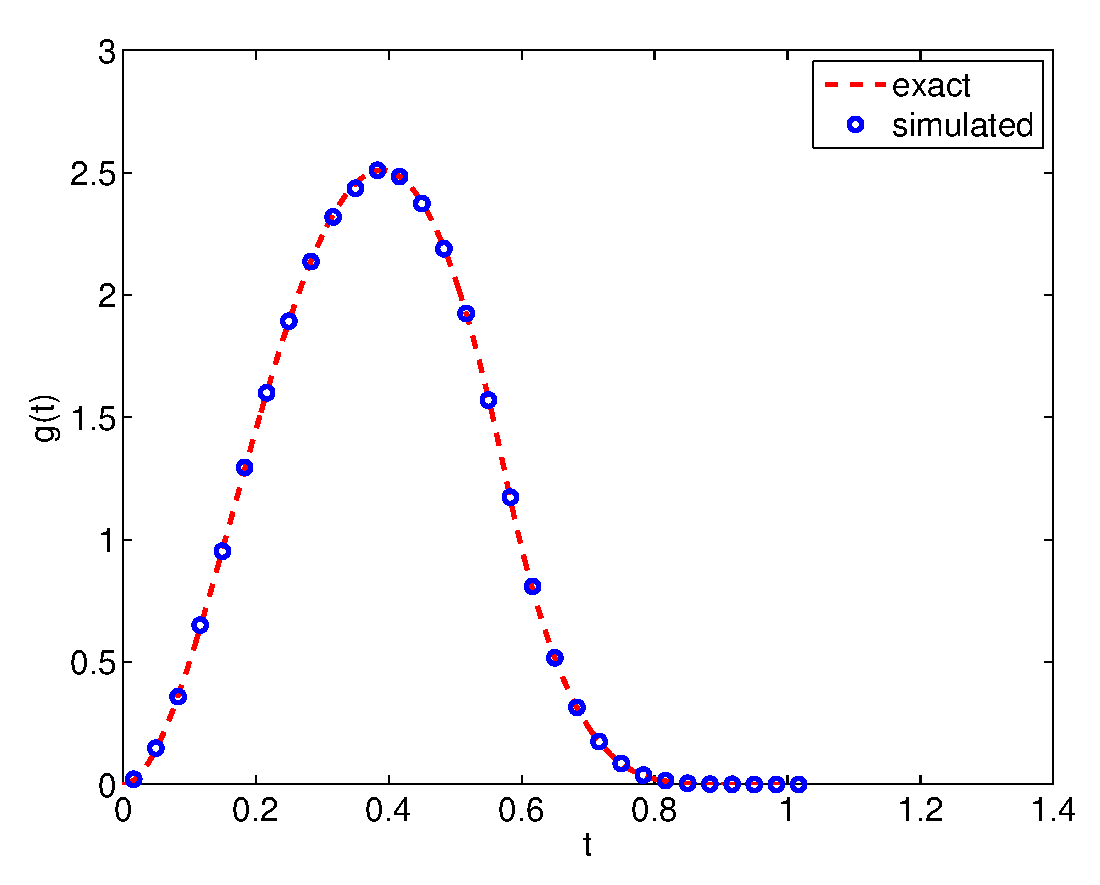
\includegraphics[width=0.32\columnwidth]{../Matlab/Plots/LinePicking_test_sim_cube.eps}} 
    \subfloat[3ball]{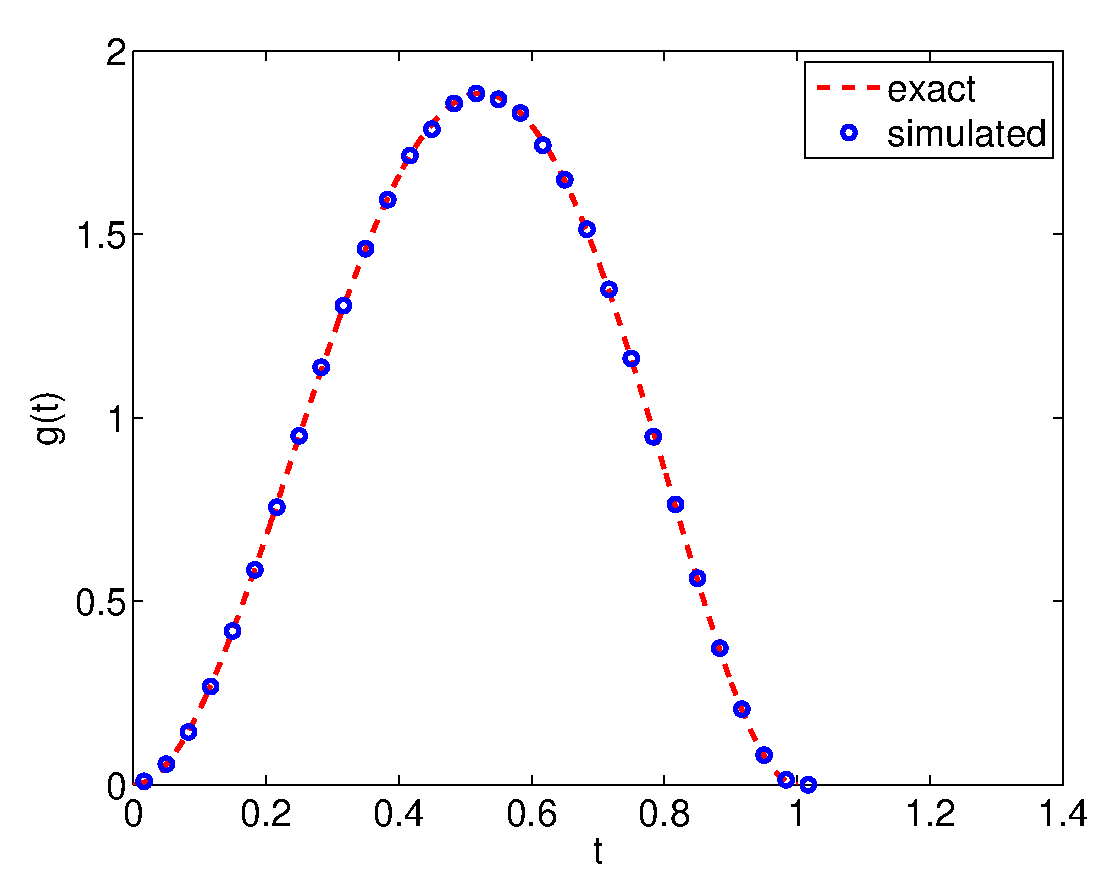
\includegraphics[width=0.32\columnwidth]{../Matlab/Plots/LinePicking_test_sim_3ball.eps}} 
    \subfloat[4ball]{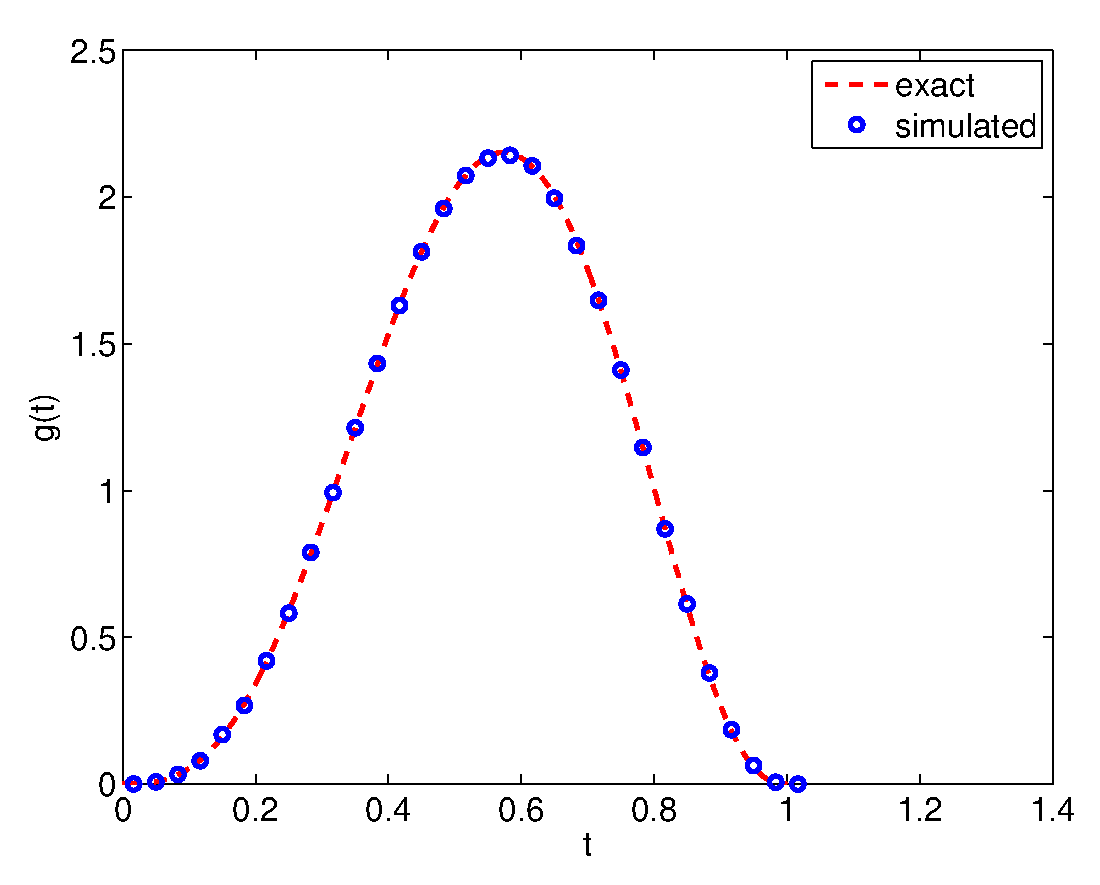
\includegraphics[width=0.32\columnwidth]{../Matlab/Plots/LinePicking_test_sim_4ball.eps}} 

    \subfloat[sphere]{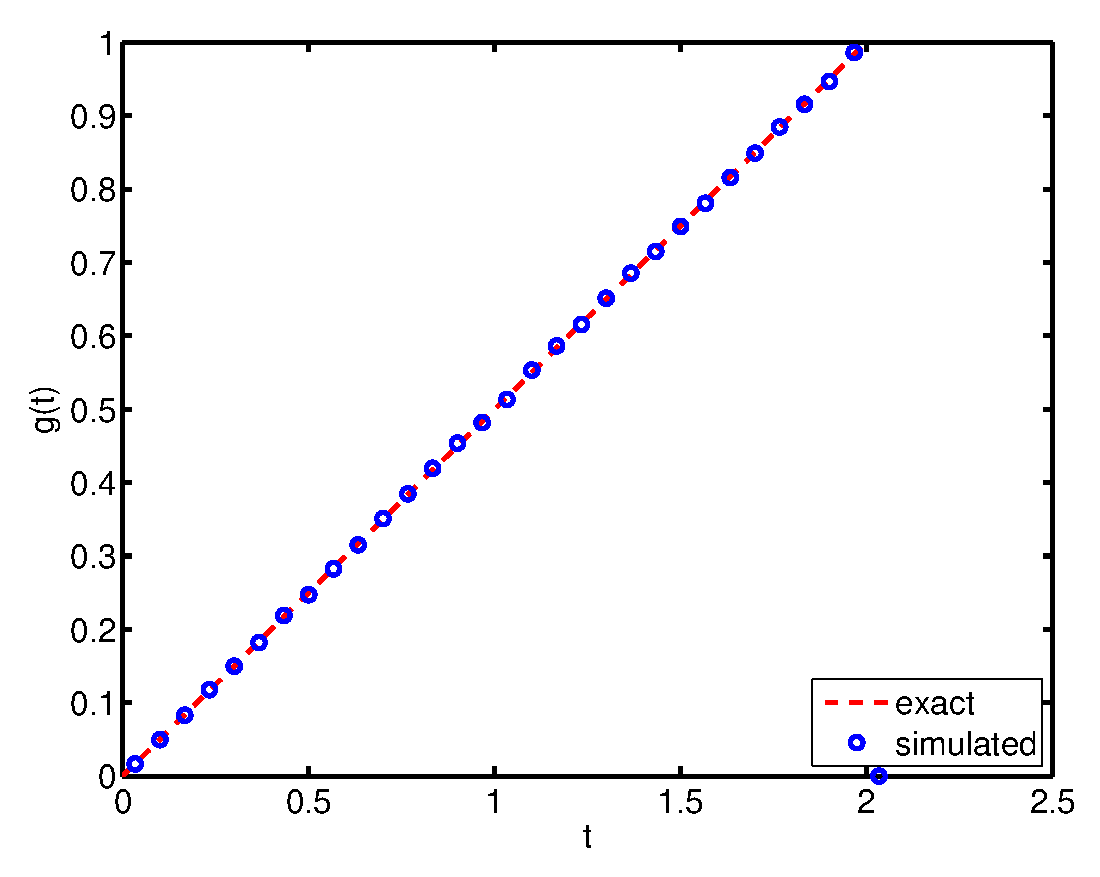
\includegraphics[width=0.32\columnwidth]{../Matlab/Plots/LinePicking_test_sim_sphere.eps}} 
    % \subfloat[sphere_geodesic]{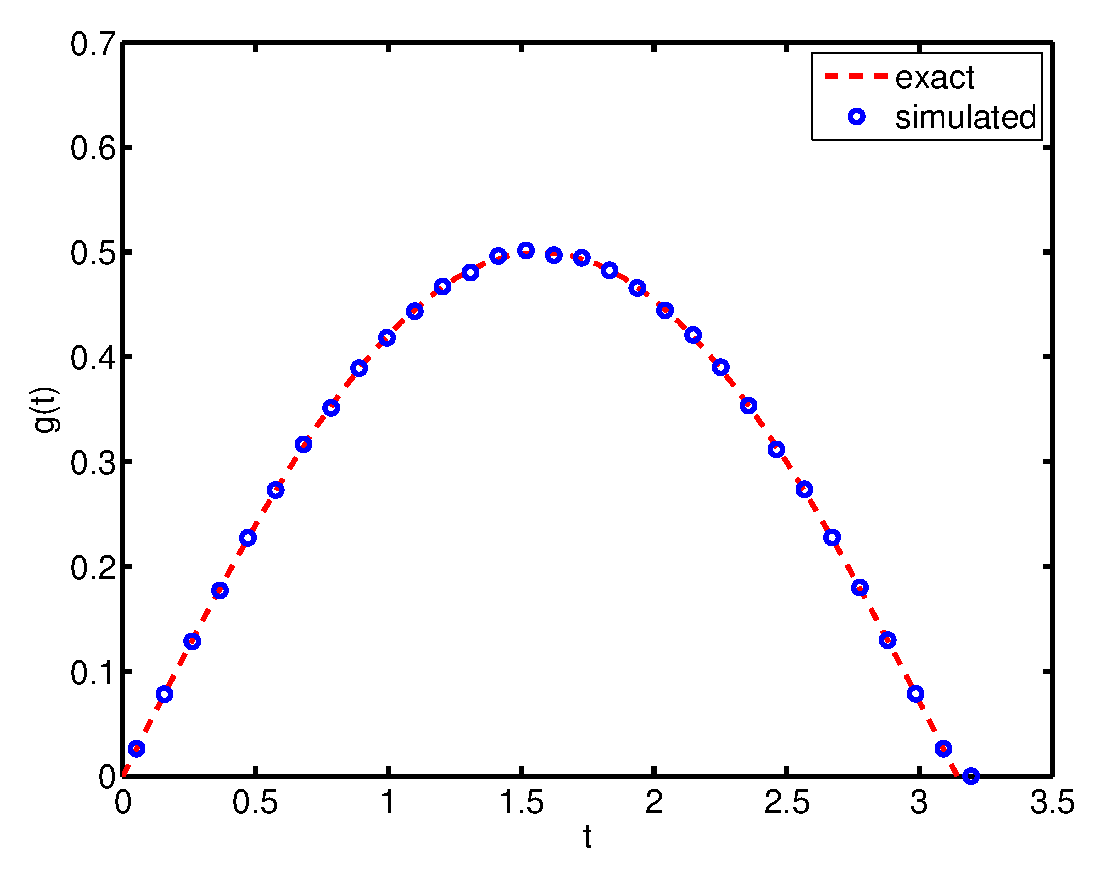
\includegraphics[width=0.32\columnwidth]{../Matlab/Plots/LinePicking_test_sim_sphere_geodesic.eps}}

    \caption{\label{fig:sim_vs_exact}Comparisons of exactly calculated distributions and the
      distributions obtained by simulation.}
  \end{center} 
\vspace{-4mm}
\end{figure}

